
%En ella se deben exponer brevemente pero con absoluta claridad, 
% la novedad y actualidad del tema,
% el objeto de la investigaci�n,
% sus objetivos,
% la hip�tesis de trabajo,
% el fundamento metodol�gico y
% los m�todos utilizados para realizar el trabajo de investigaci�n.
%Es decir, que la introducci�n es la fundamentaci�n cient�fica de la tesis en forma resumida.

\section{Introduction}
\begin{frame}
  The aim of this thesis is to support descision making concerning to
  the location and redeployment of insurance agents to attend road accidents.

  The methods of solution that will be proposed will be improve the service
  offered by insurance agents, helping them to reach in less time,
  or determine the number of unit required to perform the service within
  the desired standars.

\end{frame}

\subsection{Motivation}
\begin{frame}
  When a car accident occurs, 
  it begins to increase traffic congestion on surronding roads.
  This because the presence of an adjuster (proficient)
  which record and determine the causes of the accident,
  in order to move the car from the accident area and restore the flow.
  \begin{center}
    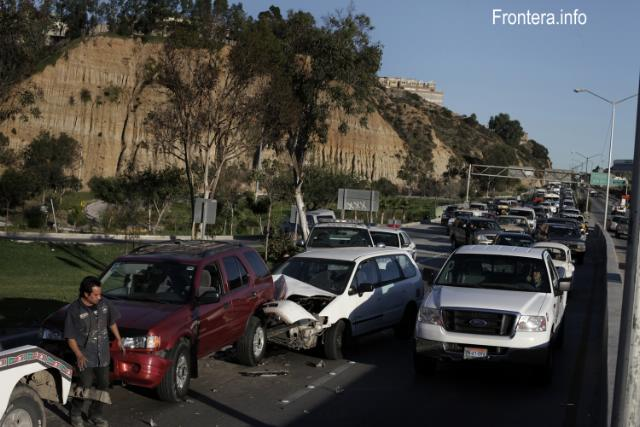
\includegraphics[scale=0.25]{389200-G}
  \end{center}
\end{frame}

\subsection{Background}
\begin{frame}
  Richard C. Larson (1974) \cite{larson1974hypercube} 
  propose the most widely referenced queueing aproachs
  for locating multiple facilities, the hypercube model.
  James P. Jarvis (1985) \cite{jarvis1985approximating} incorporate
  location dependent service times characteristics,
  developing an aproximation model for a spatially distributed queuing system
  under general service time assumptions.
\end{frame}

\begin{frame}
  Berman, Larson et. al (1987) \cite{berman1987stochastic}
  formulate the stochastic queue p-median problem,
  and propose a heuristic approach for locatin cooperative service facilities
  on a network.

  Goldberg et. al (1990) \cite{goldberg1990validating}
  propose a nonlinear integer programming
  model for finding optimal base locations for emergency medical vehicles.
  The model is described using the single objective of
  maximizing the expected number of calls served in 8 minutes.
  Stochastic travel times are considered in the objective functions
  while unequal vehicle utilization are considered in both
  the objectives and constraints.

\end{frame}
